\documentclass{memoir}
\usepackage{xcolor,color,graphicx}
\usepackage[english]{babel}
\usepackage{afterpage}
\usepackage[T1]{fontenc}
\usepackage[utf8]{inputenc}
\usepackage{palatino}
\usepackage{minted}
\usepackage{dirtree}
\usepackage[]{hyperref}
\hypersetup{
  colorlinks=true,
  allcolors={magenta},
  linkbordercolor={white},
  hypertexnames=false,
  pdftitle={reMarkable Connection Utility},
  pdfauthor={Davis Remmel},
  pdfsubject={User Manual},
  pdfkeywords={remarkable, tablet, manual, rcu, connection, utility},
  bookmarksnumbered=false,
  bookmarksopen=true,
  bookmarksopenlevel=1,
  pdfstartview=,
  pdfpagemode=UseOutlines
}

\definecolor{ared}{rgb}{.647,.129,.149}
\renewcommand\colorchapnum{\color{ared}}
\renewcommand\colorchaptitle{\color{ared}}
\chapterstyle{pedersen}

\newcommand*{\titleTH}{\begingroup% T&H Typography
  \thispagestyle{empty}
  \raggedleft
  \vspace*{\baselineskip}
  {\Large Davis Remmel}\\[0.167\textheight]
  {\textcolor{ared}{\Huge \textit{reMarkable Connection Utility}}}\\[\baselineskip]
  {\small All-in-One Local Tablet Management}\par
  \vfill{\Large User Manual}\par
  \vspace*{3\baselineskip}
\endgroup}

\makeatletter
\newcommand\footnoteref[1]{\protected@xdef\@thefnmark{\ref{#1}}\@footnotemark}
\makeatother


\begin{document}
\footnotesinmargin
\pagenumbering{roman}

\titleTH
\newpage


% Copyright Page %
\thispagestyle{empty}

\mbox{}

\vfill


\includegraphics[width=2cm]{images/cc-by-sa.png}
\vspace{0.5cm}

\small
\mbox{reMarkable Connection Utility User Manual}

\mbox{Version %%RCUFULLVER%%}

\mbox{Copyright \textcopyright{} 2020-21 Davis Remmel.}

\mbox{This manual is licensed under a \href{https://creativecommons.org/licenses/by-sa/4.0/legalcode}{Creative Commons Attribution-ShareAlike 4.0 license}.}

\mbox{\href{http://www.davisr.me/projects/rcu/}{http://www.davisr.me/projects/rcu/}}

\vspace{0.5cm}

\mbox{reMarkable\textregistered{} is a registered trademark of reMarkable AS. RCU is not affiliated with,}

\mbox{or endorsed by, reMarkable AS. The use of ``reMarkable'' in this work refers to the}

\mbox{company's e-paper tablet products.}

\vspace{0.5cm}

\mbox{macOS\textregistered{} is a registered trademark of Apple, Inc.}

\vspace{0.5cm}

\mbox{Windows\textregistered{} is a registered trademark of Microsoft, Inc.}

\newpage


\begingroup
\hypersetup{linkcolor=.}
\tableofcontents*
\endgroup
\newpage

\thispagestyle{empty}\mbox{}\newpage


\renewcommand{\thechapter}{\roman{chapter}}
\chapter{Preface}

You may have seen my work in the reMarkable tablet hacking community. I’m the one who \href{http://www.davisr.me/projects/remarkable-microsd/}{added a microSD card to the tablet}, then later installed a \href{http://www.davisr.me/projects/parabola-rm/}{desktop GNU/Linux environment}. My efforts focus on making the device usable in a general computing context.

This software, reMarkable Connection Utility (RCU), unshackles its users from\break reMarkable's proprietary cloud. The benefits are numerous: backups are low-level and full, personal notes never leave the owner's control, users may personalize their device, and the author is responsive to the needs of the community. These are things the manufacturer won't provide.

Unlike restrictive black-box software, RCU gives its users \textit{freedom}. Under the terms of its license, the \nameref{sec:license}, users hold the freedom to use it for any purpose, read the source code, modify it, share it with whomever they wish, or even re-sell it---as long as they pass forward these same freedoms. This viral licensing forms a web of non-restrictive (\textit{free}) software, leading the world toward transparency and trust, precipitating \textit{rights} for software users.

If you are a privacy-minded individual who wants to support independent software development that represents the needs of the tablet's community, please \href{http://www.davisr.me/projects/rcu/}{buy RCU}. The funds generated will support me through writing a non-proprietary handwriting recognition engine, eventually authoring ``magic paper'' software influenced by Dynabook.

I would greatly appreciate your purchase; thank you.

\vspace{1.5cm}

\rightline{Davis Remmel}
\rightline{Author of RCU}


\chapter{Support Information}
This manual, and the RCU software, are available online from the \href{http://www.davisr.me/projects/rcu/}{official project page}.

\section{General Support}

Customers of RCU's original author are entitled to some email support. The author will try his best to satisfy each customer. Please write an email using the following header fields. Please reference the PayPal transaction ID in the message body.

\vspace{0.5cm}
\begin{tabular}{rl}
To:& Davis Remmel \textless d@visr.me\textgreater \\
Subject:& RCU Support
\end{tabular}


\section{Getting Updates}

Updates for release versions are announced via email to eligible customers via email. Additionally, notices are posted to the project's \href{http://www.davisr.me/projects/rcu/}{web page} (RSS available). The program will not update automatically, but new versions may be checked for in the \nameref{sec:aboutpane}.

Customers will receive updates for 365 days from the purchase date. The program will never stop working; updates provide improvements, but a user can never be locked out of the software they own.


\section{Defect Reporting}

For users who can identify a fault with the program, and its specific circumstance of action, please submit a defect report via email with the following header fields. In the message body, please include: (a) a description of what is seen when using the program, (b) what is expected to be seen when using the program, (c) steps to reproduce the problem, and (d) information about the operating system and RCU version number (found in the \nameref{sec:aboutpane}).

\vspace{0.5cm}
\begin{tabular}{rl}
To:& Davis Remmel \textless d@visr.me\textgreater \\
Subject:& RCU Defect: \textit{Short description of problem}
\end{tabular}


\section{Mailing Lists}
There are two mailing lists: RCU-Announce, and RCU-Develop. All customers are automatically subscribed to the RCU-Announce list.

RCU-Announce is unidirectional, and only broadcasts when there are new release (stable) versions of the program. Old versions of RCU are linked in this archive.

Subscribing to RCU-Develop is optional. It is a bidirectional list meant to solicit feedback on beta features, discuss general program development, and speed up the release cycle.

\vspace{0.5cm}
\begin{tabular}{rl}
RCU-Announce& \href{https://lists.davisr.me/mailman/listinfo/rcu-announce}{https://lists.davisr.me/mailman/listinfo/rcu-announce} \\
RCU-Develop& \href{https://lists.davisr.me/mailman/listinfo/rcu-develop}{https://lists.davisr.me/mailman/listinfo/rcu-develop}
\end{tabular}
\vspace{0.5cm}

To subscribe to RCU-Develop, please write an email with the following header fields and reference the PayPal transaction ID in the message body.

\vspace{0.5cm}
\begin{tabular}{rl}
To:& Davis Remmel \textless d@visr.me\textgreater \\
Subject:& Subscribe to RCU-Develop
\end{tabular}


%% \newpage
%% \section{Contributing}
%% Since RCU is free software, users may create and share modifications. Some users may wish for their modifications to be re-incorporated into the original software.

%% The source code of RCU is distributed as a git repository. The easiest way to make contributions is to create a child branch of \textit{master}, make all the desired modifications, and then submit the diffs to the RCU Developers mailing list. The following sequence must be followed for any changes to be accepted into the official RCU software.

%% \begin{enumerate}
%% \item{Starting with the official RCU source code, which is a \textit{git} repository, checkout a new branch.}

%% \item{Make changes, and log all commits with relevant details. Commit messages should contain a concise title and descriptive body, explaining not only a summary of the changes, but also why the changes were made. Each commit should be digestible and not change more than 250 lines.}

%% \item{While under the new branch, export commits as individual patch files with \textit{git format-patch master}.}

%% \item{Send an email to the RCU Developers mailing list with the subject, ``Code Submission: \textit{Some Descriptive Title}``. In the message body, summarize the changes. The patch files should be attached to the message, not appearing in-line with the body.}

%% \end{enumerate}

%% The author watches this mailing list for all submissions. Others are encouraged to create a discussion around submissions. There is no guarantee that submissions will be accepted. Small submissions have a higher chance of being accepted.

%% \subsection{Developer Mailing List}
%% Anyone may subscribe to the developer mailing list by sending an email with the following headers.

%% \vspace{0.5cm}
%% \begin{tabular}{rl}
%% To:& RCU Developers \textless xx@example.com\textgreater \\
%% Subject:& Subscribe
%% \end{tabular}
%% \vspace{0.5cm}

%% Mailing list archives are available online at http://XXX, through which subscription preferences may also be managed.

\setcounter{chapter}{0}
\renewcommand{\thechapter}{\arabic{chapter}}
\chapter{Introduction}
\pagenumbering{arabic}
\setcounter{page}{1}

RCU allows complete offline management of a reMarkable tablet, without the need to connect with the manufacturer's proprietary cloud.

\section{Compatibility}
\label{sec:compatibility}
\begin{tabular}{ r | l }
  Hardware & reMarkable 1 \& 2 \\
  Software & 1.8.1.1--2.9.1.236 \\
  PC & FreeBSD 13.0, Ubuntu 18/20 LTS, Fedora 33, openSUSE 15.2, CentOS 7, \\
  & macOS 10.13, Windows 10 \\
\end{tabular}


\section{System Requirements}
RCU will likely run under any OS released since 2017, and its hardware requirements are minimal. It requires at-minimum 100 megabytes of disk space, and may use up to 250 megabytes of memory during some operations.

\section{Running RCU}
\label{sec:running-rcu}
RCU may connect to a tablet by USB or Wi-Fi. During periods of data transfer, never disconnect the tablet; doing so may result in a corrupted transfer.

It is possible to upload a Recovery OS with RCU, which provides an emergency SSH connection over USB and allows the user to take or restore backups of their RM1 (not RM2) device. For this recovery OS to boot, one must grant USB access under GNU/Linux and Windows, as detailed below in \nameref{sec:linnotes} and \nameref{sec:winnotes}.

RCU is distributed as a single binary package. It does not need to be installed and will run from any directory. Running RCU is as easy as double-clicking on its executable icon \footnote{macOS users must \textit{Right-Click, Open} if they have Gatekeeper enabled and are running RCU for the first time. RCU is provided with PGP signatures which ought to be used, instead of Gatekeeper, to verify authenticity.}.

RCU stores application data in the following locations.

\begin{itemize}
\item{FreeBSD, GNU/Linux}
  \begin{itemize}
  \item[]{Settings: \textit{\textasciitilde/.config/davisr/rcu.conf}}
  \item[]{Shared data: \textit{\textasciitilde/.local/share/davisr/rcu}}
  \end{itemize}
\item{macOS}
  \begin{itemize}
    \item[]{Settings: \textit{\textasciitilde/Library/Preferences/rcu.plist}}
    \item[]{Shared data: \textit{\textasciitilde/Library/Application Support/rcu}}
  \end{itemize}
\item{Windows}
  \begin{itemize}
  \item[]{Settings: \textit{HKEY\_CURRENT\_USER\textbackslash SOFTWARE\textbackslash davisr\textbackslash rcu}}
  \item[]{Shared data: \textit{\%APPDATA\%\textbackslash davisr\textbackslash rcu}}
  \end{itemize}
\end{itemize}

\newpage
\section{Entering Recovery Mode}
\label{sec:enteringrecoverymode}
An RM1 tablet may be placed into a recovery/flash mode with this sequence. If necessary, RCU can make and restore backups without there being a functional operating system. This mode is also necessary to install the Windows \textit{libusb} driver.

\begin{enumerate}
\item{Turn the device off.}
\item{Hold the middle facial button while turning the device on with the power button.}
\item{Continue holding the middle facial button for five seconds. The display will not update, but it is on.}
\item{The tablet should appear on the PC as \textit{SE Blank MERGEZ}. It is now in recovery mode.}
\end{enumerate}

When done, restart the tablet by holding the power button for 10 seconds; release, then press the power button to turn it on normally.


\section{Notes about GNU/Linux}
\label{sec:linnotes}
In order to use low-level backup/restore with RM1 devices, GNU/Linux hosts must grant read and write access to the tablet via \textit{udev}. While in recovery mode, the tablet appears as a different USB device than normal operation.

Create a new udev ruleset at \textit{/etc/udev/rules.d/50-remarkable.rules}, as shown in Figure \ref{fig:udevrules}. Replace the \textit{GROUP} attribute with a group belonging to the host's user. After creating this file, reboot the host computer.

\begin{figure}[h]
\begin{minted}[
  mathescape,
  linenos,
  numbersep=5pt,
  gobble=0,
  frame=lines,
  framesep=2mm,
  fontsize=\footnotesize]{text}
SUBSYSTEM=="usb", ATTRS{idVendor}=="15a2", ATTRS{idProduct}=="0061", \
  MODE="0660", GROUP="yourgroup"
SUBSYSTEM=="usb", ATTRS{idVendor}=="15a2", ATTRS{idProduct}=="0063", \
  MODE="0660", GROUP="yourgroup"
\end{minted}
\caption{\textit{/etc/udev/rules.d/50-remarkable.rules}}
\label{fig:udevrules}
\end{figure}

\subsection{Running on non-Ubuntu GNU/Linux}
RCU works under many GNU/Linux distributions, even if a binary is not distributed for any specific platform. The most-common incompatibility of a binary version is that PySide2 (Qt) targets a different version of \textit{glibc}, forming symbol lookup errors.

A user with non-Ubuntu GNU/Linux may need to buld their own binary, or run the program from source. This is simple with \textit{make all} or \textit{make run}, and covered further in \nameref{sec:developing}.


\newpage
\section{Notes about Windows}
\label{sec:winnotes}
In order to use low-level backup/restore with RM1 devices, Windows hosts must use the \textit{libusb-win32} driver. Distributed with the RCU binary is a copy of \href{https://zadig.akeo.ie/}{Zadig}, a utility that makes it simple to install this driver. First, the tablet must first be placed into recovery mode, which will appear as a new type of USB device.

\begin{enumerate}
  \item{Connect the tablet to a PC with USB.}
\item{Put the tablet into recovery mode by following the steps in \nameref{sec:enteringrecoverymode}.}
\item{Open Zadig}
  \begin{enumerate}
  \item{From the \textit{Options} menu, enable \textit{List All Devices}.}
  \item{In the device list, select \textit{SE Blank MERGEZ}.}
  \item{Set the driver target to \textit{libusb-win32}.}
  \item{Click \textit{Install Driver} and wait for it to complete.}
  \end{enumerate}
\item{Hold the tablet's power button for 10 seconds; release, and press it again to turn the tablet on normally.}
\item{Reboot the PC}
\end{enumerate}

\vfill

\begin{figure}[h]
  \centering
  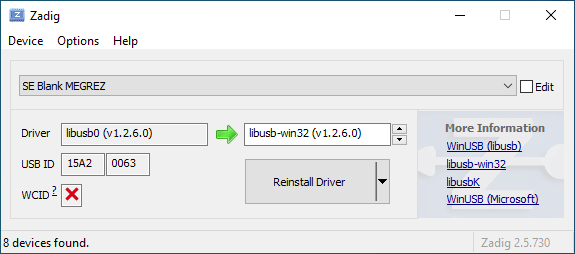
\includegraphics[width=\linewidth]{images/zadig-windows.png}
  \caption{Installing the \textit{libusb-win32} driver for Windows}
  \label{fig:zadigwindows}
\end{figure}

\vfill







\newpage
\chapter{Basic Operation}
RCU is organized into separate panes, each handling a dedicated task. Panes may be switched by clicking on their titles in the left sidebar.

\section{Connection Dialog}
\label{sec:connectiondialog}
When RCU is launched, it will show the Connection Dialog. The user must enter the information used to connect to their tablet. These configuration settings may persist by clicking the Save button. Clicking the Connect button will initiate a connection to the device\footnote{RCU uses SSH for all its communication with the tablet.} and load the Panes window.

Figure \ref{fig:connectiondialog} shows the Connection Dialog window.

\begin{figure}[h]
  \centering
  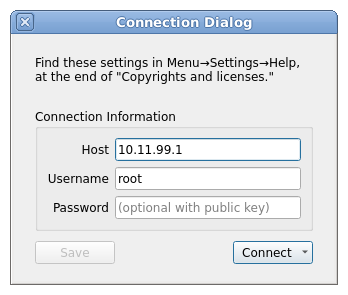
\includegraphics[width=6cm]{images/new-connection.png}
  \caption{\nameref{sec:connectiondialog}}
  \label{fig:connectiondialog}
\end{figure}

Connection presets may be stored, for using RCU with multiple devices, or on multiple networks. Presets are accessed through the small arrow on the Save button. New presets may be added, or the active preset renamed, saved, or deleted.

\begin{figure}[h]
  \centering
  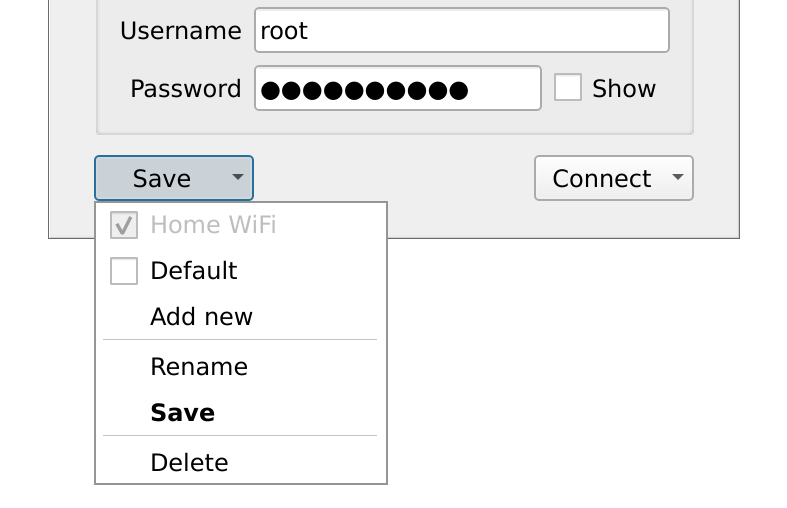
\includegraphics[width=6cm]{images/connection-presets.png}
  \caption{Access presets in the Save button drop-down menu.}
  \label{fig:cxpresets}
\end{figure}



\newpage
If a user finds themselves with an unresponsive RM1 tablet, they may place their device into a recovery mode by holding down the home button while pressing the power button. Expand the \textit{Connect} button by pressing the arrow, then click \textit{Enter Recovery OS} (Figure \ref{fig:recoveryos}) to boot over USB.\footnote{If the tablet has previously loaded the recovery OS, clicking this menu item will enter the existing recovery session.}

\begin{figure}[h]
  \centering
  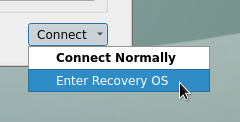
\includegraphics[width=6cm]{images/recoveryos.png}
  \caption{Enter Recovery OS}
  \label{fig:recoveryos}
\end{figure}



\newpage
\section{Device Info Pane}
\label{sec:deviceinfo}
This pane shows the user basic information about their tablet, and allows the creation and restoring of tablet backups.

\subsection{Rename}
An owner may sign their name to their tablet using the Rename button. This will change the the label from reading \textit{Connected reMarkable} to \textit{Name's reMarkable} in the \nameref{sec:deviceinfo}. This name will also be used in the author field of PDF highlight annotations (if enabled).

%% \begin{figure}[v]
%%   \centering
%%   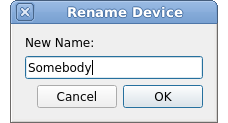
\includegraphics[width=3cm]{images/rename-dialog.png}
%%   \caption{Entering a new device name}
%%   \label{fig:deviceinfo}
%% \end{figure}

%% \begin{figure}[v]
%%   \centering
%%   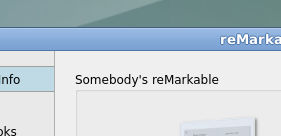
\includegraphics[width=3cm]{images/rename-label.png}
%%   \caption{Device name as it appears in \nameref{sec:deviceinfo}}
%%   \label{fig:backuprestore}
%% \end{figure}

\begin{figure}[h]
\centering
\begin{minipage}{.5\textwidth}
  \centering
  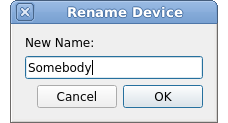
\includegraphics[height=2.5cm]{images/rename-dialog.png}
  %% \caption{Entering a new device name}
\end{minipage}%
\begin{minipage}{.5\textwidth}
  \centering
  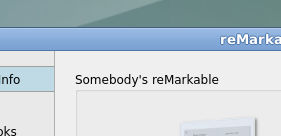
\includegraphics[height=3cm]{images/rename-label.png}
  %% \caption{Device name as it appears in \nameref{sec:deviceinfo}}
\end{minipage}
\caption{Entering a new device name}
\end{figure}


\subsection{Low-Level Backups}
There are three backup types: OS-only, Data-only, and Full. Backups may only be taken or restored through a USB connection. Only Full backups may be used to restore a bricked device.\footnote{Low-level backups only available for RM1. Users of RM2 should use \textit{Ctrl+A}, \textit{Download} in the \nameref{sec:notebookspane} to take document-level archives instead.}

OS backups will restore the operating system partitions to the tablet's internal storage. These cannot be used to restore a bricked device. If a user applies an undesired OS update to their tablet, an OS backup may be used to downgrade to the prior OS without losing data. However, there can be no guarantee the data will remain compatible with the old OS image, such as when reMarkable's system software was updated from version 1 to 2. A copy of the bootloader is captured with an OS backup.

Data backups will restore the data partition, where user documents (notebooks and uploaded files) and application settings (WiFi networks, passwords and codes) reside, to the tablet's internal storage. They will not affect the operating system partitions, and are best used to revert a bulk of documents to an earlier state.

Full backups, as seen in Figure \ref{fig:backuprestore}, may be used to restore a bricked device should the need ever arise. They require the most storage space on the client PC because they contain a complete mirror of the tablet's internal storage. A Full backup may be restored completely, or used to restore only the OS, or used to restore only the Data, or used to restore the bootloader.

The backups created in this pane are block-level, not file-level, meaning they may only be restored to the device as they were taken. Although it is possible for advanced users to extract individual files from these backups, RCU cannot. If a user finds themselves in this situation, they may refer to the \nameref{sec:backuparchiveformat}.

A custom backup directory may be set by modifying the \textit{share\_path} variable in RCU's settings (see \nameref{sec:running-rcu} for OS-specific locations).


\newpage
\mbox{}
\vfill
\begin{figure}[h]
  \centering
  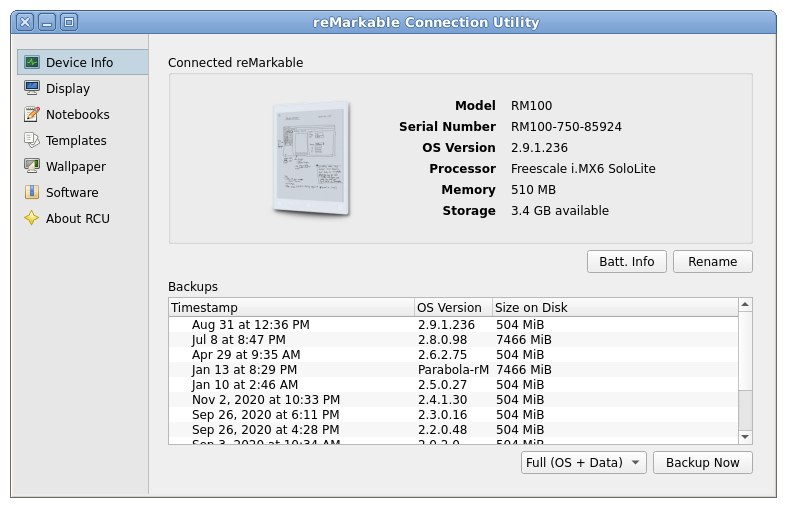
\includegraphics[width=\linewidth]{images/device-info.png}
  \caption{\nameref{sec:deviceinfo}}
  \label{fig:deviceinfo}
\end{figure}

\vfill

\begin{figure}[h]
  \centering
  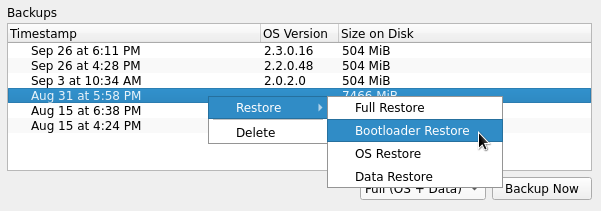
\includegraphics[width=\linewidth]{images/backup-restore.png}
  \caption{A Full backup may be restored completely, only the bootloader, only the OS partitions, or only the Data partition.}
  \label{fig:backuprestore}
\end{figure}

\vfill

\newpage
\section{Display Pane}
\label{sec:displaypane}
A user may capture screenshots of their tablet through the Display Pane. Press the Refresh button to preview the screen, then press the Save Screenshot button to record the image to disk. The image orientation may be rotated 90 degrees by choosing between the \textit{Portrait} and \textit{Landscape} radio buttons.

Although the tablet's framebuffer encodes the image as 16-bit RGB (RGB565), it is saved to disk as an 8-bit grayscale PNG, 1404$\times$1872 pixels with no transparency.

\vfill
\begin{figure}[h]
  \centering
  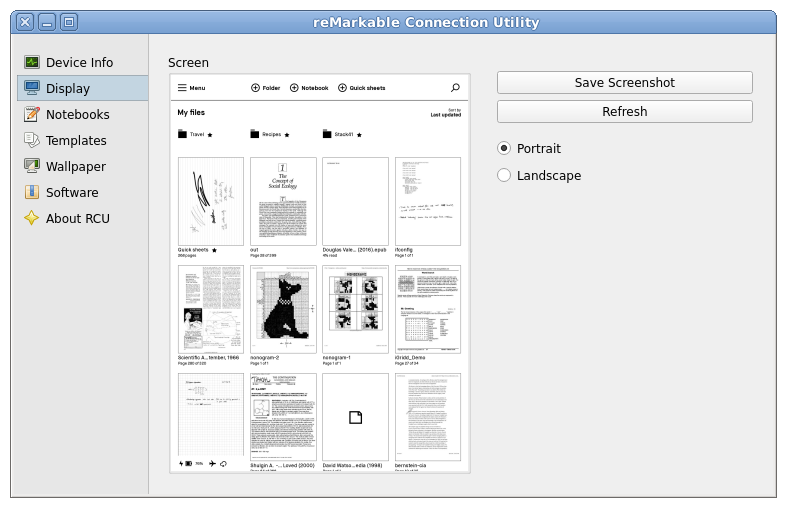
\includegraphics[width=\linewidth]{images/display.png}
  \caption{\nameref{sec:displaypane}}
  \label{fig:displaypane}
\end{figure}


\newpage
\section{Notebooks Pane}
\label{sec:notebookspane}
Documents may be transmitted between a tablet and PC through the Notebooks Pane. The default download type is a reMarkable Notebook Archive (RMN) because it can perfectly restore notebooks and their templates\footnote{Information about the RMN format may be found under \nameref{sec:notebookarchiveformat}.}.

Documents may be uploaded to the device as RMN, PDF, or EPUB files. Click the Upload button to select the file(s) to upload.

Documents may be downloaded from the device as RMNs, or exported as PDFs. It is recommended to archive notebooks with the RMN format because they are lossless, containing all the information needed to recreate a PDF. When downloading a single file, it may be renamed before it is saved. When downloading files as a batch the user must select a directory to save them in. When exporting a batch, if identically-named files already exist in the target directory, they will be overwritten.

Various style options may be found inside the Export PDF menu by clicking that button's arrow. These options are detailed in \nameref{sec:render-samples}.

By right-clicking on a document, operations such as Rename, Delete, or Favorite may be performed. When items are favorited, they appear with a star icon at the top of the tree view's sort.

Documents may be re-organized by dragging and dropping them into the desired collections.

The Notebooks Pane will automatically refresh when changes are made on the tablet. If one thinks the view is not updating properly, they may press Ctrl+R or F5 to force a refresh of notebook data.

\vfill

\begin{figure}[h]
  \centering
  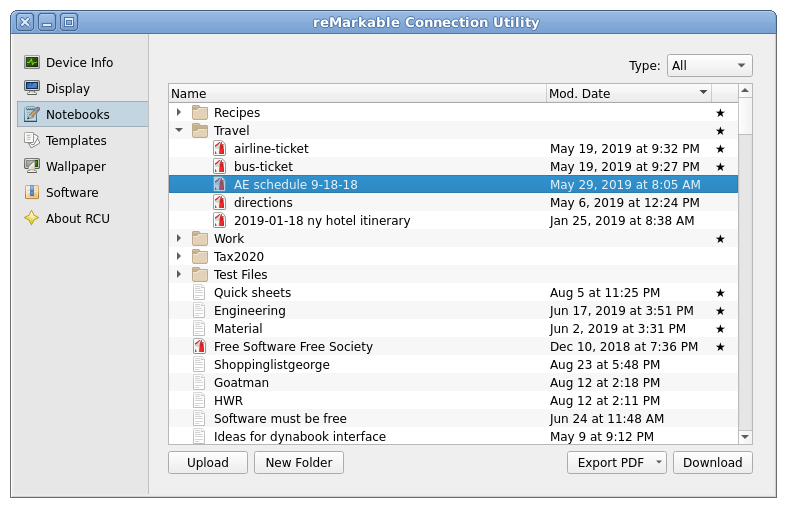
\includegraphics[width=\linewidth]{images/notebooks.png}
  \caption{\nameref{sec:notebookspane}}
  \label{fig:notebookspane}
\end{figure}

\newpage

\begin{figure}[h]
  \centering
  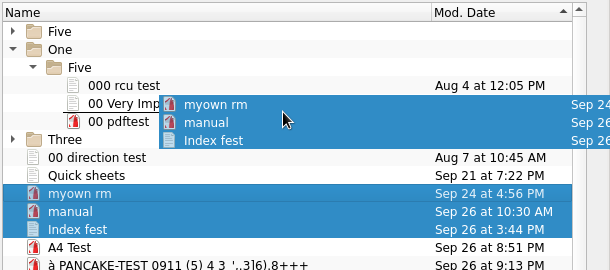
\includegraphics[width=\linewidth]{images/notebooks-dragdrop.png}
  \caption{Documents may be organized by dragging and dropping between collections.}
  \label{fig:docexport}
\end{figure}
\vfill

\begin{figure}[h]
  \centering
  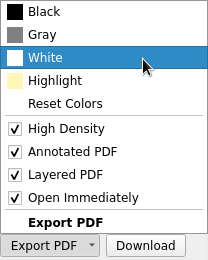
\includegraphics[height=4.5cm]{images/pdf-export-options.png}
  \caption{Choose ink colors and other \nameref{sec:render-samples}.}
  \label{fig:pdfexport}
\end{figure}
\vfill


\vfill


\begin{figure}[h]
  \centering
  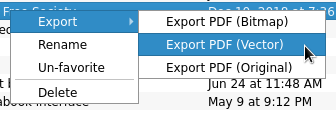
\includegraphics[height=2cm]{images/context-export.png}
  \caption{Bitmap, Vector, and Original PDF documents may be exported.}
  \label{fig:}
\end{figure}



\newpage
\section{Templates Pane}
\label{sec:templatespane}
Users may add or remove their own templates in SVG, PNG, or \nameref{sec:templatearchiveformat} (RMT). SVG or RMT formats are preferred.

Add a template to the tablet by clicking the Upload button, then selecting an RMT file. SVG and PNG templates will require the user to enter the appropriate metadata, as shown in Figure \ref{fig:templatesmodal}, and should be of appropriate resolution (1404$\times$1872 pixels).

Download a template from the tablet by selecting one in the list view, clicking the Download button, then choosing a filename to save.

Delete a template from the tablet through a contextual menu by right-clicking a template in the list view, then clicking Delete. After confirmation, RCU will permanantly delete the template from the device.

Template are installed to the user's home directory, in \textit{\textasciitilde/.local/share/remarkable/templates}. Softlinks are created where the system templates are stored, in \textit{/usr/share/remarkable/templates}. A system update may remove these links, and the templates will not load in the tablet's interface. If the user previously installed custom templates using RCU, this situation will be detected, the program will alert the user, and the template links may be restored automatically.

\vfill
\begin{figure}[h]
  \centering
  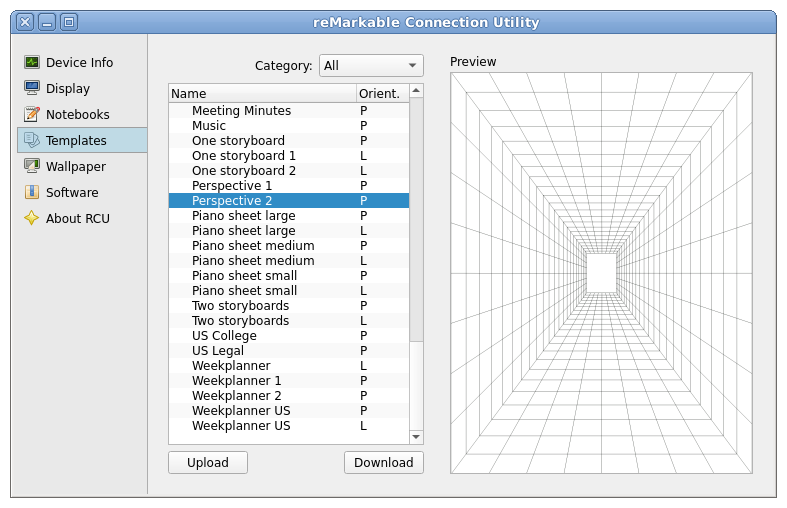
\includegraphics[width=\linewidth]{images/templates.png}
  \caption{\nameref{sec:templatespane}}
  \label{fig:templatespane}
\end{figure}

\newpage
\mbox{}
\vfill
\begin{figure}[h]
  \centering
  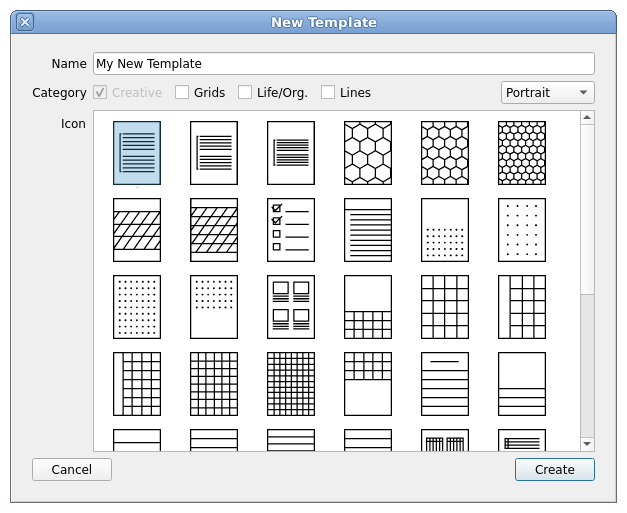
\includegraphics[width=\linewidth]{images/template-modal.png}
  \caption{\textit{New Template} modal for uploading SVG and PNG templates.}
  \label{fig:templatesmodal}
\end{figure}
\vfill


\newpage
\section{Wallpaper Pane}
\label{sec:wallpaperpane}
Device wallpapers\footnote{These are sometimes called ``splash'' images.} may be changed for the Suspend and Poweroff screens. It is recommended these images have a resolution of 1404$\times$1872 pixels, and must be in the PNG format.

The Suspend screen displays when a user taps the device's power button. Users may update this wallpaper by clicking the Upload button (beneath the Suspend label), then selecting a PNG image.

The Poweroff screen displays when a user holds the device's power button. Users may update this wallpaper by clicking the Upload button (beneath the Power Off label), then selecting a PNG image.

Images may be reset to the factory-defaults by clicking the Reset button.

\vfill
\begin{figure}[h]
  \centering
  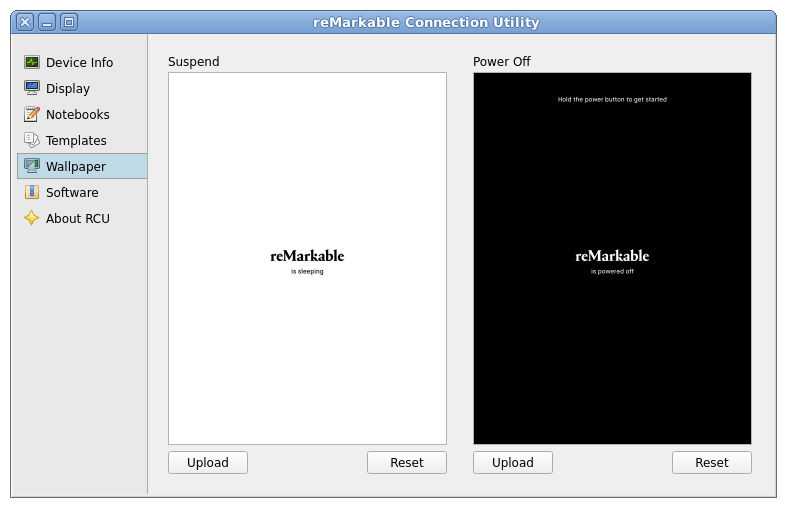
\includegraphics[width=\linewidth]{images/wallpaper.png}
  \caption{\nameref{sec:wallpaperpane}}
  \label{fig:wallpaperpane}
\end{figure}


\newpage
\section{Software Pane}
\label{sec:softwarepane}
Third-party software may be uploaded to the device in the reMarkable Software Package (RMPKG) format. For details about creating an RMPKG file, please read the \nameref{sec:softwarepackageformat}.

To install a software package, click the Upload button, select an RMPKG file, then wait for the install process to complete. RCU's interface may freeze momentarily.

To remove a software package, select one in the list view, then click the Uninstall button and wait for the removal process to complete.

\vfill
\begin{figure}[h]
  \centering
  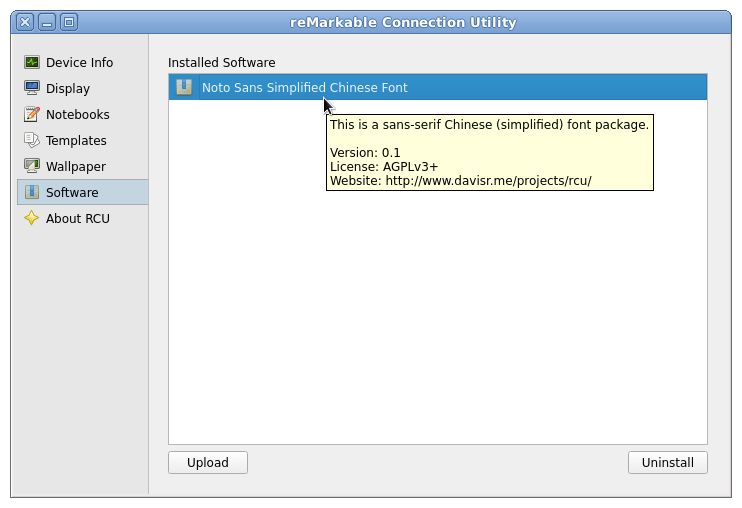
\includegraphics[width=\linewidth]{images/software.png}
  \caption{\nameref{sec:softwarepane}}
  \label{fig:softwarepane}
\end{figure}


\newpage
\section{About Pane}
\label{sec:aboutpane}
Information about RCU may be viewed in the About Pane. The information panel contains its version number. Credits to the software used to build RCU, and copies of their licenses, are also available.

By clicking the Check for Updates button, a user may request RCU to contact the update server to check if they are running the latest version.

By clicking the Fetch Compatibility button, a user may request RCU to contact the update server to download the latest compatibility table. When the reMarkable company issues a non-breaking software update, a new compatibility table allows the old version of RCU to work with the new system software version.

\vfill
\begin{figure}[h]
  \centering
  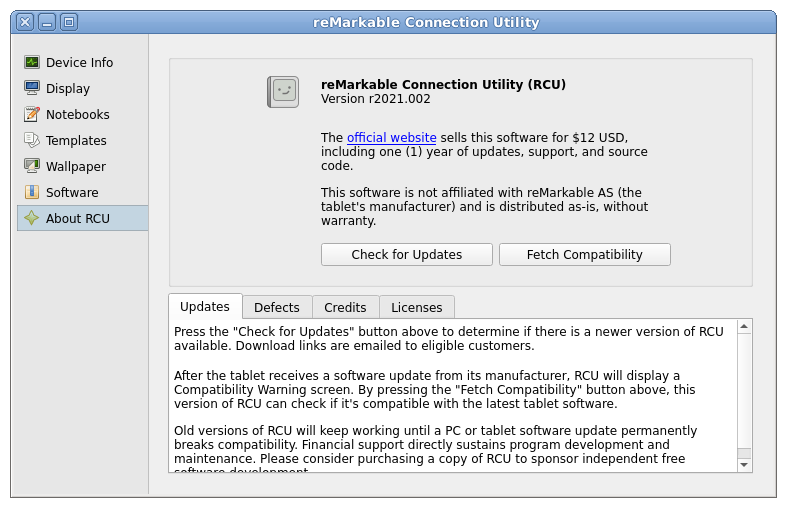
\includegraphics[width=\linewidth]{images/about.png}
  \caption{\nameref{sec:aboutpane}}
  \label{fig:aboutpane}
\end{figure}



\newpage
%%%%%%%%%%%%%%%%%%%%%%%%%%%%%%%%%%%%5
%% RENDERING SAMPLES

\chapter{PDF Export Options}
\label{sec:render-samples}



\subsection{Export Density}
RCU may export bitmap PDFs with either standard density (1404$\times$1872 pixels, \break~0.25 MB/page) or high density (2808$\times$3744 pixels, ~0.5 MB/page).

\begin{figure}[h]
\begin{tabular}{ r c c }
  Std. Density & 
\includegraphics[width=3cm]{images/export-density-standard.png}  & 
\includegraphics[width=6cm]{images/export-density-standard-2x.png}\\
  High Density & 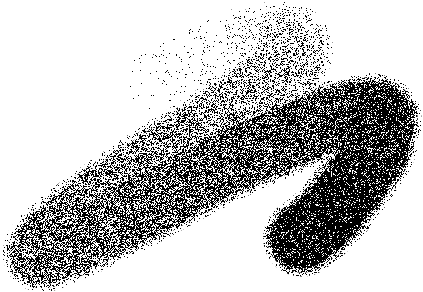
\includegraphics[width=3cm]{images/export-density-high-2x.png} & 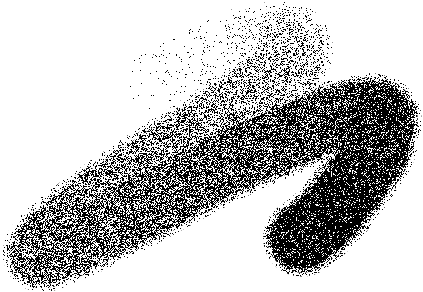
\includegraphics[width=6cm]{images/export-density-high-2x.png} \\
  \vspace{0.25cm} & \\
   & 100\% Zoom & 200\% Zoom \\
\end{tabular}
\caption{Comparison of export densities using the Pencil pen.}
\label{fig:exportdensity}
\end{figure}



\subsection{Annotations}
\label{sec:hltannot}
RCU may convert all highlight strokes to PDF highlight annotations. If using snap highlights\footnote{Snap-to-text highlights available in system software 2.7.0.51 and later.}, the highlighted text is also extracted into the annotation's comment field, as shown in Figure \ref{fig:highlightannot}. If a name is provided using the Rename button in the \nameref{sec:deviceinfo}, that name will be inserted into the anontation's author field.


\begin{figure}[h]
  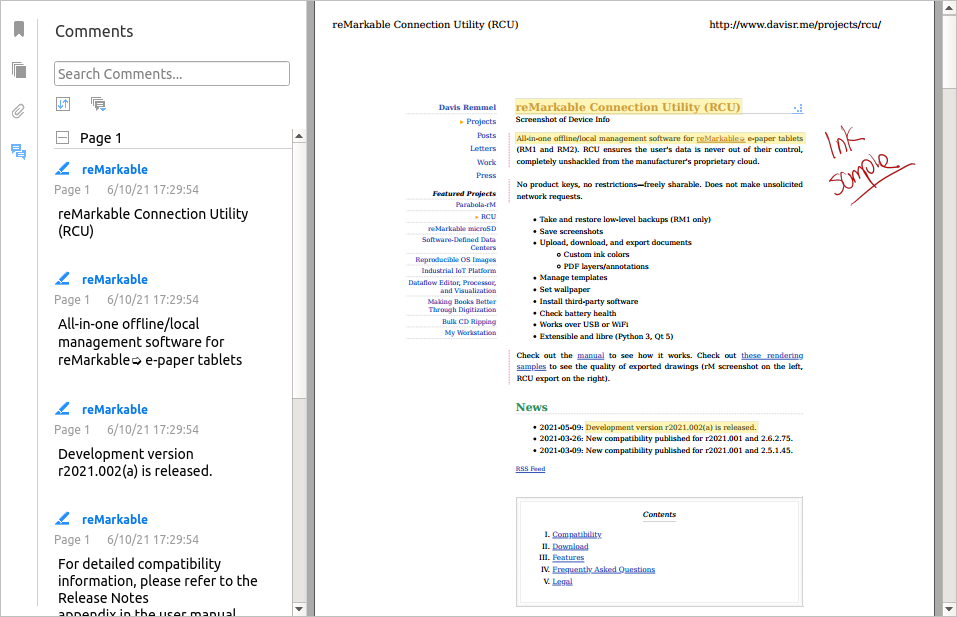
\includegraphics[width=\linewidth]{images/export-annot.png}
\caption{Exported highlight annotations shown in a PDF reader's sidebar.}
\label{fig:highlightannot}
\end{figure}





\subsection{Layers}
RCU may export each reMarkable document layer as a PDF optional content group (OCG). Most PDF readers render the OCG list into a Layers sidebar index, like shown in Figure \ref{fig:pdfocg}.


\begin{figure}[h]
  \centering
  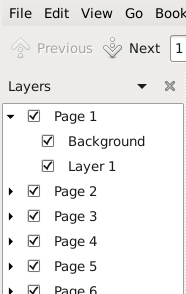
\includegraphics[width=4cm]{images/export-ocg.png}
\caption{Document layers are extracted as PDF layers.}
\label{fig:pdfocg}
\end{figure}






\newpage
\chapter{Command Line Options}
\label{sec:cli}
RCU may operate either as a GUI or a CLI program, and its behavior may be changed with flags and arguments.

\vspace{0.5cm}
\begin{tabular}{ r | c | l }
\textit{\--h}, \textit{\--\--help} & & Show help message and exit. \\
\textit{\--v}, \textit{\--\--version} & & Print version number and exit. \\
\textit{\--\--autoconnect} & & Immediately connect to last-used preset. \\
\textit{\--\--dark} & & Force dark theme. \\
\textit{\--\--no-compat-check} & & Skip pane compatibility checks (load anyway). \\
\textit{\--\--cli} & & Don't show GUI or log (best used with \textit{\--\--autoconnect}). \\
&&\\&&\\
\textit{\--\--render-rmn-pdf-b} & \textit{in.rmn \hspace{0.2cm} out.pdf} & Render local RMN archive to PDF (bitmap). \\
\textit{\--\--render-rmn-pdf-v} & \textit{in.rmn \hspace{0.2cm} out.pdf} & Render local RMN archive to PDF (vector). \\
&&\\&&\\
\textit{\--\--screenshot-p}  & \textit{out.png} & Save a screenshot as PNG (portrait). \\
\textit{\--\--screenshot-l} & \textit{out.png} & Save a screenshot as PNG (landscape). \\

\textit{\--\--list-documents} & & Tab-separated list of documents (\textit{doc\_id}, \textit{name}, and \textit{modification date}). \\
\textit{\--\--list-collections} & & Tab-separated list of collections (\textit{col\_id}, \textit{name}, and \textit{modification date}). \\

\textit{\--\--upload-doc} & \textit{in.pdf} & Upload document. \\
\textit{\--\--upload-doc-to} & \textit{in.pdf \hspace{0.2cm} col\_id} & Upload document to specific collection. \\
\textit{\--\--download-doc} & \textit{doc\_id \hspace{0.2cm} out.rmn} & Download RMN notebook archive. \\
\textit{\--\--export-pdf-b} & \textit{doc\_id \hspace{0.2cm} out.pdf} & Export PDF (bitmap). \\
\textit{\--\--export-pdf-v} & \textit{doc\_id \hspace{0.2cm} out.pdf} & Export PDF (vector). \\
\textit{\--\--export-pdf-o} & \textit{doc\_id \hspace{0.2cm} out.pdf} & Export PDF (original). \\


\end{tabular}



\section{Example Usage}


\subsection{Export a specific document as a bitmap PDF.}
\begin{enumerate}
\item{Find the ID of the document.}
  \begin{enumerate}
  \item[]{\textit{./rcu \--\--autoconnect \--\--cli \--\--list-documents}}
  \end{enumerate}
\item{Use that ID to export a PDF.}
  \begin{enumerate}
  \item[]{\textit{./rcu \--\--autoconnect \--\--cli \--\--export-pdf-b ``<doc\_id>'' ``/tmp/out.pdf''}}
  \end{enumerate}
\end{enumerate}


\subsection{Upload a document to the root folder.}
\textit{./rcu \--\--autoconnect \--\--cli \--\--upload-doc ``/tmp/in.pdf''}


\subsection{Convert an RMN to bitmap PDF without connecting to the tablet.}
\textit{./rcu \--\--render-rmn-pdf-b ``/tmp/in.rmn'' ``/tmp/out.pdf''}









\newpage
\chapter{Developing with RCU}
\label{sec:developing}
RCU is a program which is written for Python 3.6+. It uses the Qt graphics library (C++) through bindings using PySide2. Template icon (font) rendering is handled with Pillow. PDF operations are handled with Qt and Pdfrw. PC/tablet communications go through SSH using Paramiko. Although RCU is written in Python, the source and interpreter can be combined into a single executable using PyInstaller. All dependency management is handled with Python's internal virtual environment tool (venv).

Your PC should be a targeted platform (FreeBSD, GNU/Linux, macOS, or Windows). It expects to use \textit{python3.8} on FreeBSD and macOS, and will detect \textit{python\{9..6\}} on all other platforms. Python should be supportive of virtual environments using \textit{python3 -m venv}. The PC should have GNU Make and Bash (or compatible). Under Windows, the venv must be created manually inside \textit{Downloads}, and a binary must be built with \textit{Make-win.bat} instead of \textit{Makefile}.

To build the binary, run \textit{make}. Most targets utilize a Python venv, automatically created at \textit{rcu/venv}. Build assets may be cleaned with \textit{make clean}. The venv and documentation are not usually cleaned, so remove them with \textit{make clean-venv} and \textit{make clean-doc}.

\section{Common Makefile Targets}
\label{sec:makefile}

\begin{tabular}{ r | l }
  \textit{all} & Build just the binary for the current platform (default target). \\
  \textit{run} & Run the program from source within venv. \\
  \textit{venv} & Create the python venv for dependency management. \\
  \textit{doc} & Compile the user manual as PDF (requires \LaTeX). \\
  \textit{package} & Build the release archive for the current platform. \\
  \textit{clean} & Purge build assets (but keep venv and documentation). \\
\end{tabular}




\section{Adding Custom Panes}
\label{sec:devcustompanes}
The pane architecture of RCU is modular, so new panes are straightforward to add. To write a new pane, first create a new directory under \textit{src/panes} to hold the new pane's code. In that directory, create a file, \textit{pane.py}, which will serve as the focal point of execution.

The \textit{pane.py} file must contain a class for the pane, implementing the following requirements: (a) the pane must inherit from the \textit{UIController} class\footnote{\raggedleft Find the \linebreak UIController source code at \textit{src/controllers/UIController.py}.}, (b) it must provide the \textit{name} and \textit{ui\textunderscore filename} class variables, and (c) it must initialize first through the parent class. An example is listed in Figure \ref{fig:examplepanesource}.

The pane must be accompanied by a Qt UI file, specified in the class variable \linebreak\textit{ExamplePane.ui\textunderscore filename}. This is exposed to the pane's class as \textit{self.window} upon instantiation.

After adding the \textit{pane.py} file, import it within \textit{src/panes/\textunderscore \textunderscore init\textunderscore \textunderscore.py} (Figure \ref{fig:examplepaneimport}). Once added, the pane will draw itself into RCU's main window.

For non-immediate tasks, it is recommended to use a Worker object. RCU's GUI runs on the main thread, and blocking this may provide a poor user experience. Workers may be executed in the thread pool, which return to the main thread via asynchronous callback. For examples of worker usage, please read a bundled pane's code.


\begin{figure}[h]
\begin{minted}[
  mathescape,
  linenos,
  numbersep=5pt,
  gobble=0,
  frame=lines,
  framesep=2mm,
  fontsize=\footnotesize]{python}
'''
pane.py
This is an example pane.

License: AGPLv3 or later
'''

import log
from Worker import worker
from pathlib import Path
from controllers import UIController

class ExamplePane(UIController):
    name = 'Example Pane'

    # Dynamic path loading works when running from source
    # and binary.
    adir = Path(__file__).parent.parent
    bdir = Path(__file__).parent
    ui_filename = Path(adir / bdir / 'example.ui')

    xochitl_versions = [
        '^2\.2\.0\.[0-9]+$'
    ]

    @classmethod
    def get_icon(cls):
        ipathstr = str(Path(cls.bdir / 'icons' / 'emblem-documents.png'))
        icon = QIcon()
        icon.addFile(ipathstr, QSize(16, 16), QIcon.Normal, QIcon.On)
        return icon

    def __init__(self, pane_controller):
        super(type(self), self).__init__(
            pane_controller.model, pane_controller.threadpool)
        # Exposed now are self.model, self.window, and
        # self.threadpool.
        # ...
\end{minted}
\caption{Example source code for \textit{pane.py}}
\label{fig:examplepanesource}
\end{figure}

\begin{figure}[h]
\begin{minted}[
  mathescape,
  linenos,
  numbersep=5pt,
  gobble=2,
  frame=lines,
  framesep=2mm,
  fontsize=\footnotesize]{python}
  from .example.pane import ExamplePane

  paneslist = [
      # ...
      ExamplePane
      ]
\end{minted}
\caption{Example of importing \textit{pane.py} in \textit{src/panes/\textunderscore \textunderscore init\textunderscore \textunderscore.py}}
\label{fig:examplepaneimport}
\end{figure}












\chapter{Troubleshooting}
\label{sec:troubleshooting}

\subsection{RCU can't connect to the tablet.}
If a connection between the PC and reMarkable can't be established, the Connection Dialog will show an error message.

The most-common problem is trying to use incorrect login information. This information is found on the tablet, in \textit{Menu}--\textit{Settings}--\textit{Help}--\textit{Copyrights and licenses}, under the section titled \textit{GPLv3 Compliance}. If using a USB connection, the Host will be \textit{10.11.99.1}, the Username will be \textit{root}, and the Password will vary depending on the tablet. The font used to show this password can be confusing if certain characters are used, such as uppercase ``I'', lowercase ``L'', and number ``1''. Try different combinations if your password contains these characters.

If you are certian the login information is correct, it is recommended to use \textit{ping} to see if your PC is able to communicate with the tablet. Another way to test network connectivity is to enable the USB web interface, under \textit{Menu}--\textit{Settings}--\textit{Storage}. If you can connect using the web interface, you likely don't have a network problem.

If you use a PC supplied by an employer, they may be blocking network requests. In that case, it is best to speak with the IT department about granting access.


\subsection{RCU is showing a Compatibility Warning screen.}
When a reMarkable tablet receives an update to the latest firmware, RCU may display a Compatibility Warning screen. Since RCU trails reMarkable updates, it defaults to block access if using the program with a reMarkable system software version it doesn't know about. This mechanism is to prevent RCU from clobbering the tablet if reMarkable had introduced a breaking update.

If a tablet update is found to be non-breaking, then RCU does not need to be wholly updated. Instead, RCU can download a new compatibility table that will allow it to work with new tablet software. This table may be updated in the \nameref{sec:aboutpane} with the Fetch Compatibility button.

\subsection{Templates aren't included with exported notebooks.}
If a compatibility warning is bypassed for the \nameref{sec:notebookspane}, but not for the \nameref{sec:templatespane}, then templates will not be included in PDF or RMN exports. Both panes must be loaded for templates to become exported.

\subsection{macOS won't run RCU because it's from an unidentified developer.}
Most macOS users have a program called Gatekeeper enabled. This software prevents unsigned-by-Apple software from running. In order to run RCU for the first time on macOS, users typically need to \textit{Right-Click}--\textit{Open}--\textit{Open}, which will allow the user to run the program. After doing that once, a user may simply double-click on the RCU icon thereafter.

The author of RCU, instead of using Apple-specific technology, includes a platform-agnostic PGP signature to verify authenticity. If RCU was downloaded using HTTPS from \textit{files.davisr.me}, then it is safe to run.






\newpage
\appendix

\chapter{Backup Archive Format}
\label{sec:backuparchiveformat}
Low-level backups are stored on the PC's disk under RCU's shared data directory. The exact path for each operating system is listed in \nameref{sec:compatibility}.

Each backup archive is given a unique identifier, and a directory is created to store its contents. An example directory structure is listed in Figure \ref{fig:backupstructure}

\begin{figure}[h]
  \dirtree{%
  .1 backups.
  .2 902b512b-8742-481d-b5f1-e185c0668e9f.
  .3 files.
  .4 mmcblk1boot0.bin.
  .4 mmcblk1boot1.bin.
  .4 mmcblk1.bin.
  .3 backup.json.
}
\caption{Example structure of a backup archive}
\label{fig:backupstructure}
\end{figure}

The \textit{backup.json} file contains metadata about the backup, and is used by RCU to populate the UI. In summary, this file contains the backup's ID, timestamp, device information, the device's partition table (output of \textit{fdisk -l}), and checksums of the dumped partitions.

OS backups store the bootloader, secondary boot partition (containing factory device information), the bootloader data partition, primary OS partition, and secondary OS partition. The primary OS may reside on \textit{mmcblk1p2} or \textit{mmcblk1p3}, flipping after every system update.

\begin{itemize}
\item{/dev/mmcblk1boot0}
\item{/dev/mmcblk1boot1}
\item{/dev/mmcblk1p1}
\item{/dev/mmcblk1p2}
\item{/dev/mmcblk1p3}
\end{itemize}

Data backups only store the data partition, which is mounted as \textit{/home/root}.

\begin{itemize}
\item{/dev/mmcblk1p7}
\end{itemize}

Full backups store the bootloader, secondary boot partition, and the entire contents of the eMMC (all partitions combined).

\begin{itemize}
\item{/dev/mmcblk1boot0}
\item{/dev/mmcblk1boot1}
\item{/dev/mmcblk1}
\end{itemize}


\chapter{Notebook Archive Format}
\label{sec:notebookarchiveformat}
Notebook Archive (RMN) files contain the raw editable data used by Xochitl, plus a copy of each template applied. They have an obvious structure, as seen in Figure \ref{fig:rmnstructure}. This directory is a direct export from Xochitl's files, from the device at \textit{\textasciitilde/.local/share/remarkable/xochitl}.

\begin{figure}[h]
  \dirtree{%
    .1 ExampleNotebook.rmn.
    .2 6bde82bd-f580-456b-8275-c853438707a6/.
    .3 5ae652c8-280b-4b00-9563-72f25f16ac29.rm.
    .3 3e9610c9-7633-4964-8198-adc0d1968cea.rm.
    .3 (...).
    .2 6bde82bd-f580-456b-8275-c853438707a6.highlights/.
    .2 6bde82bd-f580-456b-8275-c853438707a6.bookmarks.
    .2 6bde82bd-f580-456b-8275-c853438707a6.content.
    .2 6bde82bd-f580-456b-8275-c853438707a6.metadata.
    .2 6bde82bd-f580-456b-8275-c853438707a6.pagedata.
    .2 Blank.rmt.
    .2 Small Lines.rmt.
}
\caption{Example structure of a template archive}
\label{fig:rmnstructure}
\end{figure}

When saving a document it is preferred to use the RMN format over the PDF format because RMN files contain an exact copy of those notebooks. Therefore, a PDF may always be generated from an RMN archive.\footnote{See: \nameref{sec:cli}}

Notebook archive files store all templates used in the document. When uploading an archive to a new device, these templates will be automatically installed if they didn't already exist.


\chapter{Template Archive Format}
\label{sec:templatearchiveformat}
The Template Archive (RMT) format stores a vector image and reMarkable UI metadata in a single file. Typically, reMarkable templates are shared as singular PNG images; this has a number of drawbacks, like being stuck with a static resolution and lack of metadata.

The RMT format solves those issues by bundling a vector image of the template (SVG), instead of a bitmap image, and includes template metadata (JSON) in a tape-archive (TAR). An example file structure of an RMT file may be seen in Figure \ref{fig:rmtstructure}.

\begin{figure}[h]
  \dirtree{%
    .1 ExampleTemplate.rmt.
    .2 template.json.
    .2 template.svg.
}
\caption{Example structure of a template archive}
\label{fig:rmtstructure}
\end{figure}

The \textit{template.json} file should contain, at minimum, a structure similar to Figure \ref{fig:exampletemplatejson}. The \textit{fileName} attribute should be a UUID and is necessary to prevent template collisions; if this is not explicitly specified, one will be generated by RCU.\footnote{Do not share manually-created RMT files that don't have a \textit{fileName} attribute, otherwise collisions may occur or there could be multiple versions of identical templates.} The \textit{categories} array may contain any of the following strings:

\begin{itemize}
\item{Creative}
\item{Grids}
\item{Life/organize}
\item{Lines}
\end{itemize}


\begin{figure}[h]
\begin{minted}[
  mathescape,
  linenos,
  numbersep=5pt,
  gobble=2,
  frame=lines,
  framesep=2mm,
  fontsize=\footnotesize]{json}
  {
      "categories": [
          "Creative"
      ],
      "iconCode": "\ue9d5",
      "landscape": false,
      "name": "Example Template",
      "fileName": "<UUID>"
  }
\end{minted}
\caption{Example source code for \textit{template.json}}
\label{fig:exampletemplatejson}
\end{figure}

The \textit{template.svg} file should contain valid SVG data and have a viewport resolution of 1404$\times$1872 pixels. When a template archive is uploaded, these files are not extracted to the default template location (\textit{/usr/share/remarkable/templates}). Instead, they are extracted into the user's home directory at \textit{\textasciitilde/.local/share/remarkable/templates}. Upon upload, RCU will convert the SVG image to a PNG image to retain compatibility with Xochitl.

If the tablet receives an update that clears the system template directory, the templates will become unavailable from the interface. RCU may detect this condition and prompt the user to recreate these template links, in-effect restoring the templates (they do not need to be re-uploaded).

\chapter{Software Package Format}
\label{sec:softwarepackageformat}
Please download the RCU sources, then find the \textit{rmpkg-sample} directory. This sample package contains lots of useful information about the package format in a practical way, by using a self-extracting shell script with a tape-archive payload.

The RMPKG format is a self-contained executable that exposes a number of command line arguments. This format has several convenient properties:

\begin{itemize}
\item{Installable any time, directly onto a stock tablet, no other software required (not even RCU).}
\item{Self-contained package format convenient to download, convenient for authors to earn income for their work.}
\item{Possible to write an RMPKG in any language that targets ARMv7}
  \item{No Internet access required}
\item{Handles own compatibility checks, installation, and uninstallation}
  \end{itemize}


There are many ways to build a program that fit this description. The easiest way to configure an RMPKG is with an ordinary shell script, appended with the application's binary payload (like a .tar), which self-executes. An RMPKG should expose the following flags.

\begin{itemize}
\item{\textit{\phantom{}-\phantom{}-info}: Prints information about the package useful for anyone who stumbles upon it}
\item{\textit{\phantom{}-\phantom{}-manifest}: Prints a manifest of any files touched by the package; used for detecting conflicting packages}
\item{\textit{\phantom{}-\phantom{}-install}: Installs the package payload to the system}
\item{\textit{\phantom{}-\phantom{}-uninstall}: Uninstalls the package payload from the system}
\end{itemize}

RCU uploads packages to the tablet's \textit{\textasciitilde /.rmpkg} directory. %% Implement this: after performing a software update, RCU will check and reinstall each package in ~/.rmpkg.









\chapter{Release Notes}
\label{sec:releasenotes}


%%%%%%%%%%%%%%%%%%%%%%%%%%%%%%%%%%%%
\section{%%RCUFULLVER%%}
Released on September 10, 2021, this version addresses compatibility with system software 2.9.1.236, adds CLI options for transferring documents, and improves PDF handling and rendering.

\subsection{Compatibility}
\begin{tabular}{ r | l }
  Hardware & reMarkable 1 \& 2 \\
  Software & 1.8.1.1--2.9.1.236 \\
  PC & FreeBSD 13.0, Ubuntu 18/20 LTS, Fedora 33, openSUSE 15.2, CentOS 7, \\
  & macOS 10.13, Windows 10 \\
\end{tabular}

%% \subsection{Important Notices}
%% \begin{itemize}
%% \item[!]{Sample notice.}
%% \end{itemize}

\subsection{Release Notes}
\begin{itemize}
\item{Compatibility with system software 2.9.1.236, rm2fb.\footnote{This is a shim for other third-party software (not RCU) to display graphics on RM2. Read more: \textit{\href{https://github.com/ddvk/remarkable2-framebuffer}{ddvk/remarkable2-framebuffer}}.}}
  \item{Snap-highlighted text extracts into PDF highlight comments.}
  \item{High Density export option (4x DPI bitmap rendering).}
  \item{Create folders and sub-folders.}
\item{Sticky favorited documents and collections on-top.}
\item{Removed pop-up notice when connection becomes interrupted.}
  \item{Check for pseudo-deleted files and prompt non-cloud users to purge.}
    \item{New CLI options: \textit{\--\--cli}, \textit{\--\--screenshot-p}, \textit{\--\--screenshot-l}, \textit{\--\--list-documents}, \textit{\--\--list-collections}, \linebreak\textit{\--\--download-doc}, \textit{\--\--export-pdf-b}, \textit{\--\--export-pdf-v}, \textit{\--\--export-pdf-o}, \textit{\--\--upload-doc}, \linebreak\textit{\--\--upload-doc-to}, \textit{\--\--render-rmn-pdf-b}, \textit{\--\--render-rmn-pdf-v}}
    \item{Show error message for About Pane network failures.}
\item{Improved PDF handling with regards to CropBox, MediaBox.}
\item{Improved handling with reMarkable Cloud.}
\item{Bundle SSL certificates.}
  \item{Sanitize quote characters from filenames.}
\item{Fixed defect where Mechanical Pencil v1 (from system software prior to 1.8.1.1) rendered incorrectly.}
  \item{Fixed defect where RM2 screenshots were mis-aligned by 8 pixels.}
  \item{Fixed defect where using Adjust View had no effect on exported PDFs.}
  \item{Fixed defect where the recovery OS was dependent upon contents of eMMC. Tablet now shows black screen during recovery operations.}
  \item{Fixed defect where connection presets could disappear.}
  \item{Fixed defect where RMN uploads were invisible if they were originally taken from a parent folder.}
    \item{Fixed defect where the program could crash for macOS 11 (Big Sur) users when exporting select PDFs.}
    

\end{itemize}

\subsection{Known Defects}
\begin{itemize}
\item{Some documents exported with a base PDF and Layers enabled may render OK, but be reported in Adobe Acrobat as having a generic error, and the Background layer may toggle the entire page.}
\item{Improper annotation rotation with PDF pages that are rotated 270 degrees (usually appearing upside-down).}
\item{Some PDFs are unable to be decoded and fail to export, or export blank. Some examples are password-protected PDFs, and My Deep Guide's yearly planner.\footnote{A temporary workaround is to process these PDFs with \textit{qpdf} and overwrite the original PDF on the device through SSH.}}
  \item{Lucida Console is forced on macOS, instead of the default system typeface, because of a font-rendering issue in Qt with macOS 11 (Big Sur) where space characters that appear after a comma or period are invisible.}
  \item{No warning for RMPKG fault}
\end{itemize}






\newpage
%%%%%%%%%%%%%%%%%%%%%%%%%%%%%%%%%%%%
\section{r2021.001}
\label{sec:r2021.001}
Released on January 31, 2021, this version addresses compatibility for reMarkable 2, system software 2.5.0.27, and macOS Big Sur, fixes bugs and annoying behavior, and introduces new features.

\subsection{Compatibility}
\begin{tabular}{ r | l }
  Hardware & reMarkable 1 \& 2 \\
  Software & 1.8.1.1--2.5.0.27 \\
  PC & FreeBSD 12.1, Ubuntu 18/20 LTS, Fedora 33, openSUSE 15.2, CentOS 7, \\
  & macOS 10.13-11.1, Windows 10 \\
\end{tabular}

\subsection{Important Notices}
\begin{itemize}
\item[!]{Low-level backup/restore is unsupported with reMarkable 2.}
\item[!]{reMarkable 2 owners on Windows do not need to install the libusb driver.}
\end{itemize}

\subsection{Release Notes}
\begin{itemize}
\item{reMarkable 2 compatibility, screenshots}
  \item{System software 2.5.0.27 compatibility}
  \item{macOS 11 (Big Sur) compatibility}
  \item{KDE, dark theme support}
    \item{Parabola-rM backup/restore}
  \item{Directly import SVG and PNG images as templates}
  \item{Multiple presets for different networks}
  \item{Password visibility toggle}
  \item{Hierarchical download/export documents}
  \item{CLI flags: \textit{\--\--autoconnect}, \textit{\--\--dark}, \textit{\--\--no-compat-check}}
  \item{Rename documents and collections}
  \item{Application icon, GNU/Linux installers}
  \item{Fetch new compatibility tables without updating RCU}
  \item{Switches program license to GNU AGPLv3 or later}
  \item{Uses to .app packaging for macOS}
  \item{Makefile conveniences, like venv and packaging}
  \item{Keyboard shortcuts for quitting/closing}
  \item{Fixes defect where key-based authentication was used instead of password}
  \item{Fixes defect where data-only restore was non-functional}
  \item{Fixes defect where \textit{/home/root} was sometimes used instead of \textit{\$HOME}}
  \item{Fixes defect where backups under Windows failed when running RCU from a non-primary volume}
  \item{Fixes defect where upload progress meter never changed from 0\%}
\end{itemize}

\subsection{Known Defects}
\begin{itemize}
\item{Unable to load recovery OS when the tablet has a botched splash image.\footnote{A new recovery OS is available by email, but was not polished enough to make this release.}}
\item{Some documents exported with a base PDF and Layers enabled may render OK, but be reported in Adobe Acrobat as having a generic error, and the Background layer may toggle the entire page.}
\item{Force-refreshing the Notebooks Pane doesn't work under FreeBSD or macOS.}
\item{No conflict check for RMPKGs}
\item{No warning for RMPKG fault}
\end{itemize}




\newpage
%%%%%%%%%%%%%%%%%%%%%%%%%%%%%%%%%%%%
\section{r2020.003}
\label{sec:r2020-003}
Released on October 3, 2020, this version addresses compatibility for system software 2.3.0.16, fixes bugs and annoying behavior, and introduces new export options.

\subsection{Compatibility}
\footnote{This version is likely compatible with reMarkable 2 (except backup/restore) but is untested.}
\begin{tabular}{ r | l }
  Hardware & RM100, RM102 (reMarkable 1) \\
  Software & 1.8.1.1--2.3.0.16 \\
  PC & FreeBSD 12.1, Ubuntu 18.04, macOS 10.13, Windows 10 \\
\end{tabular}

\subsection{Important Notices}
\begin{itemize}
\item[!]{This version changes the settings and data paths. To migrate old backups, copy the \textit{backups} directory from the old data directory to the new one. The old data directories are:}
  \begin{itemize}
  \item[]{FreeBSD, GNU/Linux: \textit{\textasciitilde/.config/rcu}}
  \item[]{macOS: \textit{\textasciitilde/Library/Preferences}}
  \item[]{Windows: \textit{C:\textbackslash HKEY\_CURRENT\_USER\textbackslash SOFTWARE\textbackslash rcu\textbackslash rcu}}
  \end{itemize}
\end{itemize}

\subsection{Release Notes}
\begin{itemize}
\item{System software 2.3.0.16 compatibility}
\item{Resizable UI, with Hi-DPI support}
\item{New application data directory, user-setable in configuration file}
  \begin{itemize}
  \item{FreeBSD, GNU/Linux}
    \begin{itemize}
    \item[]{Settings: \textit{\textasciitilde/.config/davisr/rcu.conf}}
    \item[]{Data: \textit{\textasciitilde/.local/share/davisr/rcu}}
    \end{itemize}
  \item{macOS}
    \begin{itemize}
    \item[]{Settings: \textit{\textasciitilde/Library/Preferences/rcu.plist}}
    \item[]{Data: \textit{\textasciitilde/Library/Application Support/rcu}}
    \end{itemize}
  \item{Windows}
    \begin{itemize}
    \item[]{Settings: \textit{HKEY\_CURRENT\_USER\textbackslash SOFTWARE\textbackslash davisr\textbackslash rcu}}
    \item[]{Data: \textit{\%APPDATA\%\textbackslash davisr\textbackslash rcu}}
    \end{itemize}
  \end{itemize}
\item{Faster startup/load time}
\item{Automatic notebook view refresh (force with Ctrl+R or F5)}
\item{Drag-and-drop document organization within the Notebooks Pane}
\item{Save last-used directory for import/export operations}
\item{Save notebook sorting method}
\item{Upload to any collection (document folder)}
\item{No longer requires Host to be an IP address in the Connection Dialog}
\item{A port may be given in the Host field, separated with a ':' (colon)}
\item{New Export PDF options}
  \begin{itemize}
  \item{PDF annotations for highlights}
  \item{PDF layers (OCG) for each document layer}
  \item{Customizable ink colors}
  \item{Auto-open exported PDF}
  \end{itemize}
\item{Fix Wallpaper Pane bugs}
  \begin{itemize}
  \item{Removed "Powered Off" overlay text}
  \item{Set to Original button works as-expected and will always keep a backup}
  \end{itemize}
\item{Fix rM Cloud compatibility bugs (delete, re-uploading old archives)}
\item{Sanitize export filenames}
\item{Compatibility with more GNU/Linux distros}
  \begin{itemize}
  \item{Now requires libxcb as a dependency (install \textit{libxcb-xinerama0})}
  \end{itemize}
\item{Warning popup when the tablet is disconnected}
\item{reMy, from which RCU gets its .lines parser, is now credited visibly in the About Pane}
\item{Reduce logging verbosity}
\item{Smoother lines when exporting vectors}
\end{itemize}

\subsection{Known Defects}
\begin{itemize}
\item{Some documents exported with a base PDF and Layers enabled may report in Adobe Acrobat as having a generic error, but otherwise render OK.}
\item{Force-refreshing the Notebooks Pane doesn't work under macOS.}
\item{No conflict check for RMPKGs}
\item{No warning for RMPKG fault}
\end{itemize}



%%%%%%%%%%%%%%%%%%%%%%%%%%%%%%%%%%%%
\newpage
\section{r2020.002}
\label{sec:r2020-002}
Released on September 6, 2020, this version addresses issues blocking users from running \nameref{sec:r2020-001}.

\subsection{Compatibility}
\begin{tabular}{ r | l }
  Hardware & RM100, RM102 (reMarkable 1) \\
  Software & 1.8.1.1--2.2.0.48 \\
  PC & FreeBSD 12.1, Ubuntu 18.04, macOS 10.13, Windows 10 \\
\end{tabular}

\subsection{Release Notes}
\begin{itemize}
\item{Fix "unknown document version" bug}
\item{Fix improper handling of tall PDF documents}
\item{Warn user when not taking/restoring backup from USB}
\item{Set executable permission in macOS release archive}
\item{Update manual with recovery mode instructions}
\item{Update manual with Windows driver instructions}
\end{itemize}

\subsection{Known Defects}
\begin{itemize}
\item{No conflict check for RMPKGs}
\item{No warning for RMPKG fault}
\end{itemize}









%%%%%%%%%%%%%%%%%%%%%%%%%%%%%%%%%%%%
\newpage
\section{r2020.001}
\label{sec:r2020-001}
Released on September 5, 2020, this is the first released version of RCU.

\subsection{Compatibility}
\begin{tabular}{ r | l }
  Hardware & RM100, RM102 (reMarkable 1) \\
  Software & 1.8.1.1--2.2.0.48 \\
  PC & FreeBSD 12.1, Ubuntu 18.04, macOS 10.13, Windows 10 \\
\end{tabular}

\subsection{Release Notes}
\begin{itemize}
\item{First release of reMarkable Connection Utility (RCU)}
\item{Application will open with console window}
\end{itemize}
















%%%%%%%%%%%%%
%% LICENSE %%
%%%%%%%%%%%%%%%%%%%%%%%%%%%%%%%%%%%%

% END OF TEMPLATE %
% The makefile appends after this (see `make doc`) %
% %%%%%%%%%%%%%%%%%%%%%%%%%%% %
